\documentclass[../main.tex]{subfiles}

\begin{document}

\chapter{Формування та аналіз вимог до Android-щоденника}

\section{Формування вимог}

Розглянувши існуючі на цей час програмні продукти, такі як щоденники для мандрівників, проаналізувавши їх, та виявивши як позитивні так і негативні сторони, можна сформувати задачі розробки. В узагальненому вигляді такою задачею є створення додатку, що буде забезпечувати можливість ведення щоденнику, запису треку переміщень та планування поїздок.
При проектуванні програмного продукту необхідно забезпечити наступні можливості:

\begin{enumerate}
	\item Авторизація за допомогою Google аккаунта.
	\item Можливість створення подорожі.
	\item Можливість створення записів щоденника.
	\item Можливість створення записів планувальника.
	\item Можливість встановлення нагадувань.
	\item Можливість запису треку переміщень.
\end{enumerate}

\section{Аналіз вимог}

Аналіз вимог є частиною процесу розробки програмного забезпечення, що включає в себе збір вимог щодо програмного забезпечення, їх систематизацію, виявлення взаємозв'язків, а також документування.

\subsection{Авторизація за допомогою Google аккаунта}
Для того, щоб користувач мав доступ тільки до своїх даних, та мав можливість синхронізації з іншими пристроями, він повинен мати свій обліковий запис в базі даних. Так як в якості бази даних використовуэться Firebase, маємо такі варіанти авторизації користуваців: 
\begin{itemize}
	\item За допомогою соціальних мереж (Google, Facebook, Twitter)
	\item За допомогою аккаунта GitHub
	\item За допомогою адерси електронної пошти
	\item Анонімна авторизація
\end{itemize}

Майже всі користувачі Android-пристроїв мають аккаунт Google, тому було вирішено використовувати саме цей метод авторизації. В майбутньому можуть бути додані будь-які інші методи авторизації.

\subsection{Можливість створення подорожі}
Так як розроблюваний додаток є щоденником для мандрівників, користувач повинен мати змогу створювати подорожі. Створені подорожі слугують категоріями, в яких можуть знаходитися записи щоденника та планувальника. Також трек переміщень пов'язаний з певною мандрівкою.

\subsection{Можливість створення записів щоденника}
Користувач, який встановив Android-щоденник, очікує від нього можливість ведення йього щоденника, тому однією з головних вимог такого додатку є змога сворення записів у щоденнику. Для створення запису, користувачу не обовязково потрібно мати створені подорожі. Записи без вказаної подорожі будуть розміщуватися в загальному щоденнику.

\subsection{Можливість створення записів планувальника}
Важливим пунктом для мандрівників є планування поїздок, тому користувач повинен мати змогу створювати записи планувальника, в яких він зможе описати все, що йому потрібно зробити при плануванні подорожі.

\subsection{Можливість встановлення нагадувань}
При підготовці до подорожі важливо не забути завершити заплановані справи та зібрати необхідні речі чи документи, тому користувач повинен мати змогу встановлювати нагадування для записів планувальника. Нагадування можуть бути встановлені на конкретний час, чи по приближенню до вказаного місця.

\subsection{Можливість запису треку переміщень}
Користувач повинен мати змогу записувати трек свого переміщення. Це допоможе не забути якими маршрутами він рухався, та  які місця відвідав. Запис треку можливий при наявності активної подорожі. Для забезпечення цієї вимоги необхідно передбачити механізм запису місцезнаходження користувача в період його подорожі до бази даних.

\section{Об'єктний аналіз вимог інформаційної системи}

\subsection{Формулювання вимог за допомогою діаграми прецедентів}
На основі визначених вимог було побудовано діаграму прецедентів (див. рис. \ref{diagram:1}), яка дозволить отримати візуальне уявлення про вимоги користувачів.

\begin{figure}[H]
	\centering
	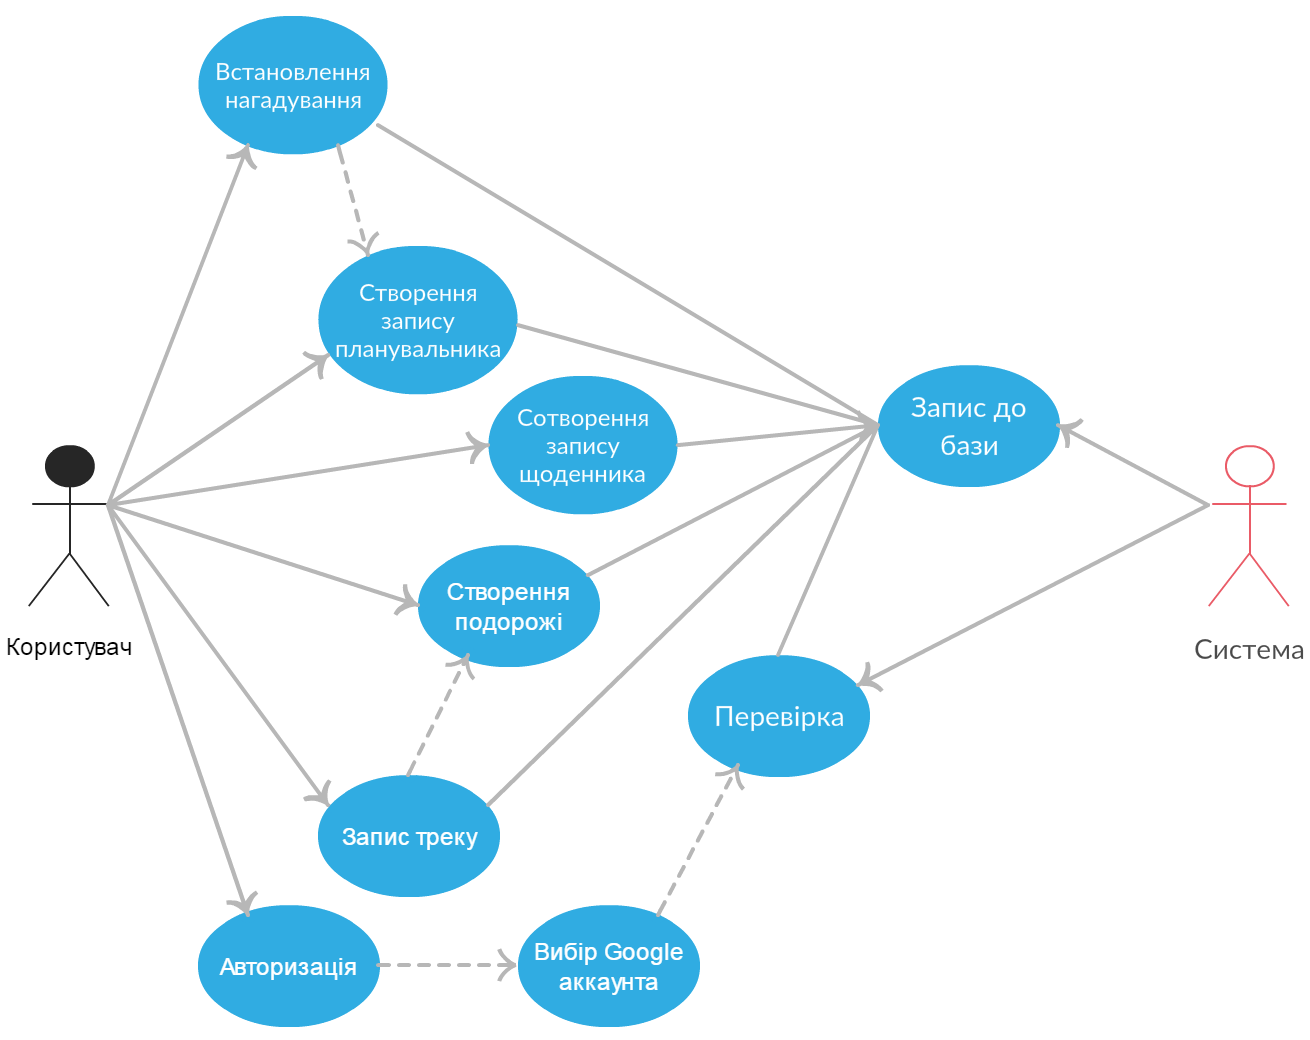
\includegraphics[width=1\textwidth]{diagram_usecase}
	\caption{Механізм роботи з додатком у вигляді діаграми прецедентів}
	\label{diagram:1}
\end{figure}

\subsection{Формулювання та аналіз вимог за допомогою діаграми діяльності}

На основі первинних вимог були розроблені наступні детальні вимоги:
\begin{enumerate}
	\item Надати можливість редагувати подорож.
	\item Надати можливість видаляти подорож.
	\item Надати можливість редагувати запис щоденника.
	\item Надати можливість видаляти запис щоденника.
	\item Надати можливість редагувати запис планувальника.
	\item Надати можливість видаляти запис планувальника.
	\item Надати можливість додавати зображення до запису щоденника.
	\item Надати можливість переглядати карту з треком і мітками.
	\item Надати можливість обирати подорож для запису щоденника та планувальника.
	\item Надати можливість встановлювати активну подорож.
	\item Надати можливість синхронізувати дані між пристроями.
	\item Надати можливість ділитися записами щоденника через інші додатки.
	\item Надати можливість ділитися окремими зображеннями з запису щоденника через інші додатки.
	\item Надати можливість додавати списки з прапорцями в запис планувальника.
	\item Надати можливість системі автоматично завантажувати дані про погодні умови та місцезнаходження при створенні запису щоденника.
\end{enumerate}

Моделюючи поведінку системи, яка проектується або проводиться її аналіз, постає необхідність деталізувати особливості алгоритмічної і логічної реалізації виконуваних системою операцій. Для такого моделювання в мові UML використовуються діаграми діяльності.

У контексті мови UML діяльність (activity) є деякою сукупністю окремих обчислень, що виконуються автоматом. При цьому окремі елементарні обчислення можуть наводити до деякого результату або дії (action). На діаграмі діяльності відображується логіка або послідовність переходу від однієї діяльності до іншої, при цьому увага фіксується на результаті діяльності. Сам же результат може привести до зміни стану системи або повернення деякого значення.

Діаграма діяльності створення нового запису щоденника, що відображає поведінку проектованої системи подана на рис. \ref{diagram:2}.

\begin{figure}[H]
	\centering
	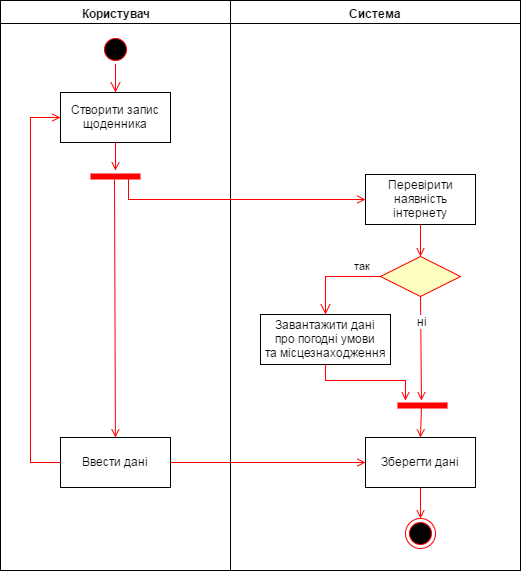
\includegraphics[width=1\textwidth]{diagram_activity}
	\caption{Механізм створення запису щоденника у вигляді діаграми діяльності}
	\label{diagram:2}
\end{figure}

% TODO: add other diagrams

\subsection{Аналіз вимог за допомогою діаграми послідовності}

\subsection{Аналіз вимог за допомогою діаграми комунікації}

\section{Визначення поведінки об'єктів системи}

% TODO: Висновки обсягом 0,5-1 с.

\end{document}